
Le baklava est une pâtisserie traditionnelle dans plusieurs pays comme la Bulgarie ou
le Maroc. Il s'agit d'un dessert long à préparer, à base de pâte feuilletée, de miel, de
noix ou de pistaches ou de noisettes, selon les régions.
Dans un sachet non transparent, on a sept baklavas indiscernables au toucher portant
les lettres du mot BAKLAVA.
\begin{center}
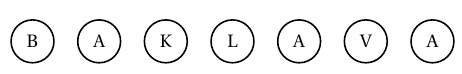
\includegraphics[scale=1]{Prob-33.png} 
\end{center}

On tire au hasard un gâteau dans ce sachet et on regarde la lettre inscrite sur le
gâteau.

\medskip

\begin{enumerate}
\item Quelles sont les issues de cette expérience ?
\item Déterminer les probabilités suivantes:
	\begin{enumerate}
		\item La lettre tirée est un L.
		\item La lettre tirée n'est pas un A.
	\end{enumerate}
\item  Enzo achète un sachet contenant $10$ baklavas tous indiscernables au toucher.
	
Ce sachet contient $2$ baklavas à base de pistaches, $4$ baklavas à base de noisettes
et les autres baklavas sont à base de noix.
	
Enzo pioche au hasard un gâteau et le mange ; c'est un gâteau à base de noix. 

Il souhaite en manger un autre.

Son amie Laura affirme que, s'il veut maintenant prendre un nouveau gâteau, il
aura plus de chances de piocher un gâteau à base de noix.

A-t-elle raison ? Justifier la réponse.
\end{enumerate}